% Poster A1 vertical (594 x 841 mm) - Seminario de Investigacion, Universidad Ean   [v2]
% BORRADOR BASE: maqueta + figuras + cifras recalculadas desde datos/resultados.csv.
% El TEXTO de los bloques es un punto de partida; reescribanlo con sus palabras (regla de IA, clase 7).
% Reglas: titulo >=72 pt, subtitulos 36-48 pt, cuerpo >=24 pt, 2 familias max, 3 colores + blanco/gris, 800-1000 palabras.
% Fotos: copiar sus fotos a poster/fotos/ con los nombres g1.jpg g2.jpg falla.jpg; si no existen se dibuja un recuadro.
\documentclass[24pt]{extarticle}
\usepackage[paperwidth=594mm,paperheight=841mm,margin=16mm]{geometry}
\usepackage[utf8]{inputenc}
\usepackage[T1]{fontenc}
\usepackage[spanish]{babel}
\usepackage{helvet}
\renewcommand{\familydefault}{\sfdefault}
\usepackage{xcolor,graphicx,tcolorbox,array,booktabs,tikz}
\usetikzlibrary{arrows.meta,calc}
\tcbuselibrary{skins}
\definecolor{navy}{HTML}{0B2A5B}
\definecolor{ambar}{HTML}{D98A00}
\pagestyle{empty}
\setlength{\parindent}{0pt}
\setlength{\parskip}{8pt}
\newcommand{\cuerpo}{\fontsize{24}{30}\selectfont}
\newtcolorbox{bloque}[2][]{enhanced,colback=white,colframe=navy,boxrule=2pt,arc=14pt,
  colbacktitle=navy,coltitle=white,fonttitle=\fontsize{44}{52}\bfseries\selectfont,halign title=center,
  title={#2},left=16pt,right=16pt,top=8pt,bottom=10pt,toptitle=5pt,bottomtitle=5pt,#1}
% foto o recuadro provisional
\newcommand{\foto}[3]{\IfFileExists{fotos/#1.jpg}{\includegraphics[width=#2,height=#3,keepaspectratio]{fotos/#1.jpg}}{%
  \begin{tikzpicture}\draw[ambar,very thick,dashed,rounded corners=6pt] (0,0) rectangle (#2,#3);
  \node[ambar,font=\fontsize{24}{28}\bfseries\selectfont,align=center] at (#2/2,#3/2) {FOTO\\ #1};\end{tikzpicture}}}
% pieza dibujada: capas horizontales, eje de la pieza girado a #1 grados respecto de la cama, flecha = carga
\newcommand{\orient}[2]{\begin{tikzpicture}[scale=1.25]\pgfmathsetmacro{\sh}{1.5*sin(#1)+0.05}
  \fill[navy!8] (-2.2,-0.35) rectangle (2.2,0); \draw[thick] (-2.2,0) -- (2.2,0);
  \begin{scope}[shift={(0,\sh)}]
    \clip[rotate=#1] (-1.5,0) rectangle (1.5,0.7);
    \foreach \y in {-2,-1.75,...,2.5}{\draw[navy!55,line width=1.1pt] (-3,\y) -- (3,\y);}
  \end{scope}
  \begin{scope}[shift={(0,\sh)},rotate=#1]
    \draw[navy,line width=2.2pt,rounded corners=2pt] (-1.5,0) rectangle (1.5,0.7);
    \draw[ambar,line width=3pt,-{Stealth[length=7pt]}] (1.5,0.35) -- (2.25,0.35);
    \draw[ambar,line width=3pt,-{Stealth[length=7pt]}] (-1.5,0.35) -- (-2.25,0.35);
  \end{scope}
  \node[font=\fontsize{24}{28}\bfseries\selectfont] at (0,-0.75) {#2};
\end{tikzpicture}}
\begin{document}
\cuerpo
% ---------------- TITULO ----------------
\begin{tcolorbox}[enhanced,colback=navy,colframe=navy,arc=0pt,left=22pt,right=22pt,top=14pt,bottom=14pt,
  overlay={\node[anchor=south east,inner sep=10pt,text width=40mm,align=center,font=\fontsize{20}{24}\selectfont\color{white}] at (frame.south east) {
\includegraphics[width=34mm]{qr_articulo.png}\\[2pt]Artículo (PDF)};}]
\centering\color{white}
{\fontsize{72}{80}\bfseries\selectfont Orientación y configuración FDM: comportamiento mecánico de piezas de PLA con diseño generativo\par}
\vspace{8pt}
{\fontsize{30}{36}\selectfont Alisson Dayana Navarro Rodriguez\par}
{\fontsize{26}{32}\selectfont Universidad Ean $\bullet$ Facultad de Ingeniería $\bullet$ Bogotá, Colombia $\bullet$ anavarr36555@universidadean.edu.co\par}
\end{tcolorbox}
\vspace{3mm}
% ---------------- 1 + 2 ----------------
\noindent\begin{minipage}[t]{0.485\linewidth}\vspace{0pt}
\begin{bloque}{1 | Problema}
\cuerpo
Una pieza FDM no es un sólido homogéneo: su resistencia depende de cómo se depositan las capas. El diseño generativo permite obtener geometrías optimizadas, pero su desempeño real depende de las condiciones de fabricación FDM.\par
\begin{tcolorbox}[colback=ambar!12,colframe=ambar,boxrule=3pt,arc=8pt,left=8pt,right=8pt,top=4pt,bottom=4pt]
\textbf{Pregunta.} ¿Cómo influyen la orientación, la configuración de impresión y la geometría generativa en la fuerza máxima, la deformación y la masa de piezas de PLA en tensión, compresión y flexión?
\end{tcolorbox}
\end{bloque}
\end{minipage}\hfill
\begin{minipage}[t]{0.485\linewidth}\vspace{0pt}
\begin{bloque}{2 | Metodología}
\cuerpo
\centering\fontsize{25}{30}\selectfont
\textbf{Fusion 360} $\rightarrow$ \textbf{Creality Print} $\rightarrow$ \textbf{PLA} $\rightarrow$ \textbf{ensayos} $\rightarrow$ \textbf{análisis}\par
\raggedright\fontsize{24}{30}\selectfont
Seis piezas (G1 y G2 por ensayo) con tres configuraciones \emph{combinadas} y tres orientaciones: 54 probetas, una por condición. 215\,°C, cama 60\,°C. Carga manual progresiva hasta la falla, medida con celda de carga (axial, vertical y central en viga apoyada).\par
\centering\fontsize{23}{28}\selectfont
\begin{tabular}{@{}lcccc@{}}\toprule
 & Relleno & Paredes & Capa & Patrón\\\midrule
Fina & 15\,\% & 2 & 0,12 mm & Cúbico\\
Estándar & 15\,\% & 2 & 0,20 mm & Cúbico\\
Fuerte & 25\,\% & 5 & 0,20 mm & Giroide\\\bottomrule
\end{tabular}\par
\end{bloque}
\end{minipage}
\vspace{3mm}
% ---------------- 3 PIEZAS Y ORIENTACION ----------------
\begin{bloque}{3 | Piezas generativas y orientación de capas}
\centering\cuerpo
\foto{g1}{104mm}{58mm}\hfill\foto{g2}{78mm}{58mm}\hfill
\orient{0}{0°}\hfill\orient{45}{45°}\hfill\orient{90}{90°}\par
\vspace{2pt}
{\fontsize{22}{26}\selectfont Laminado en Creality Print \quad$\bullet$\quad Piezas impresas \quad$\bullet$\quad Orientación: capas en azul, carga en naranja.\par}
\end{bloque}
\vspace{3mm}
% ---------------- 4 RESULTADOS ----------------
\begin{bloque}{4 | Resultados}
\centering\cuerpo
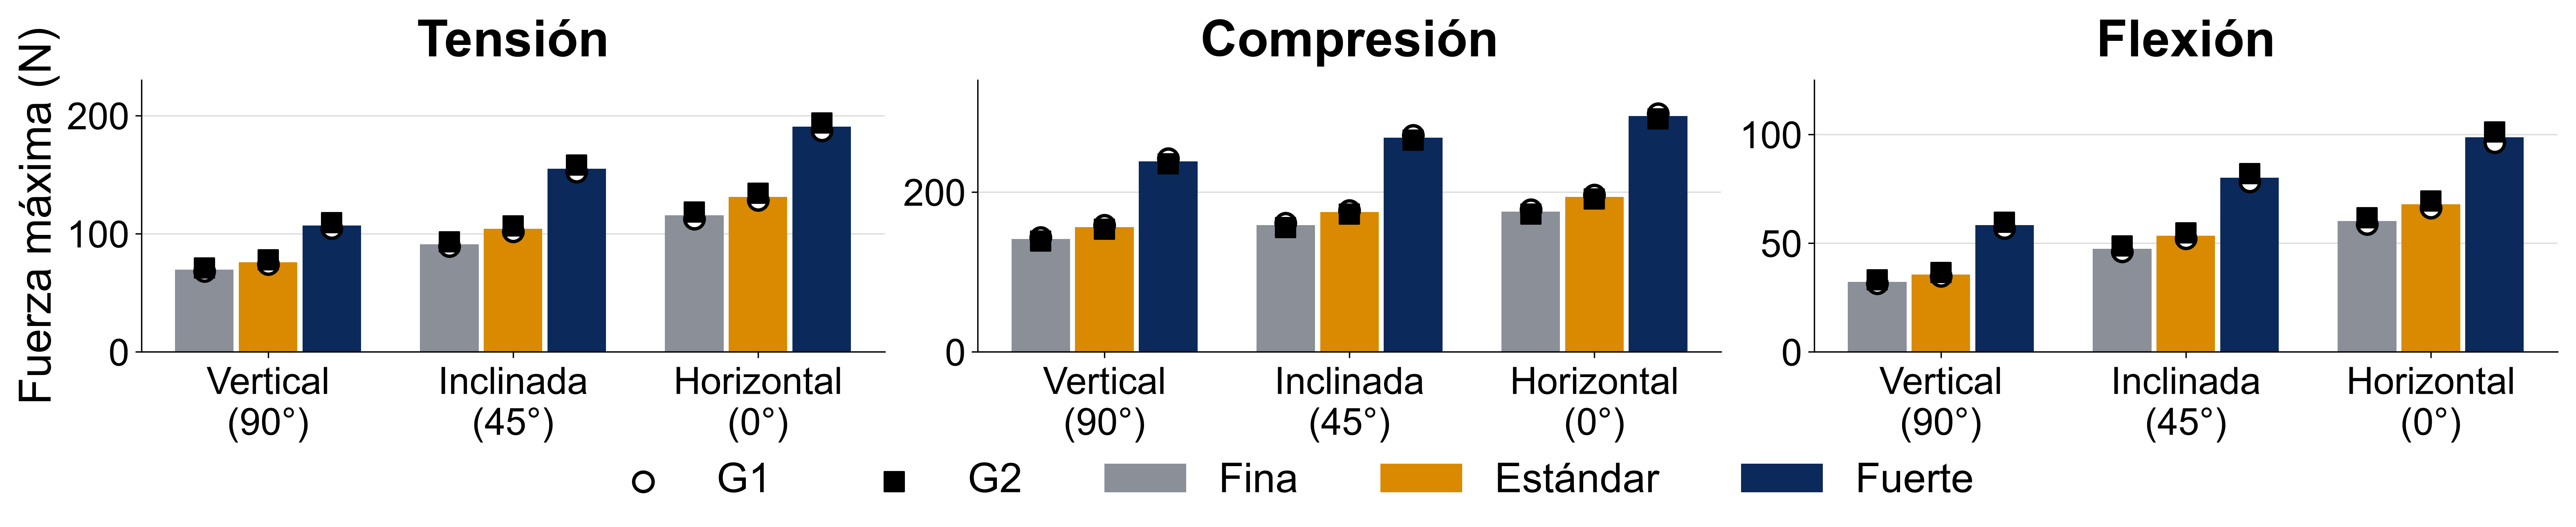
\includegraphics[width=0.97\linewidth]{../figuras/fig1_fmax_poster.png}\par
{\fontsize{22}{26}\selectfont\textit{Figura 1.} Fuerza máxima por configuración y orientación (barra: media de G1 y G2; círculo: G1; cuadrado: G2). n = 1 por condición.\par}
\vspace{4pt}
\begin{minipage}[c]{0.56\linewidth}\raggedright\fontsize{25}{32}\selectfont
\textbf{Carga.} Fuerte soporta 64--70\,\% más fuerza que Fina (razón de medias de 18 probetas por configuración), con 109\,\% más masa (9,1 g contra 4,3 g).\par
\textbf{Orientación.} La horizontal dio la mayor carga en los tres ensayos; la vertical queda 42\,\% (tensión), 19\,\% (compresión) y 45\,\% (flexión) por debajo. En tensión y flexión la vertical falló por delaminación intercapa; en compresión, por pandeo o aplastamiento.\par
\textbf{Geometría.} G1 y G2 difieren menos de 6\,\%.
\end{minipage}\hfill
\begin{minipage}[c]{0.42\linewidth}\centering
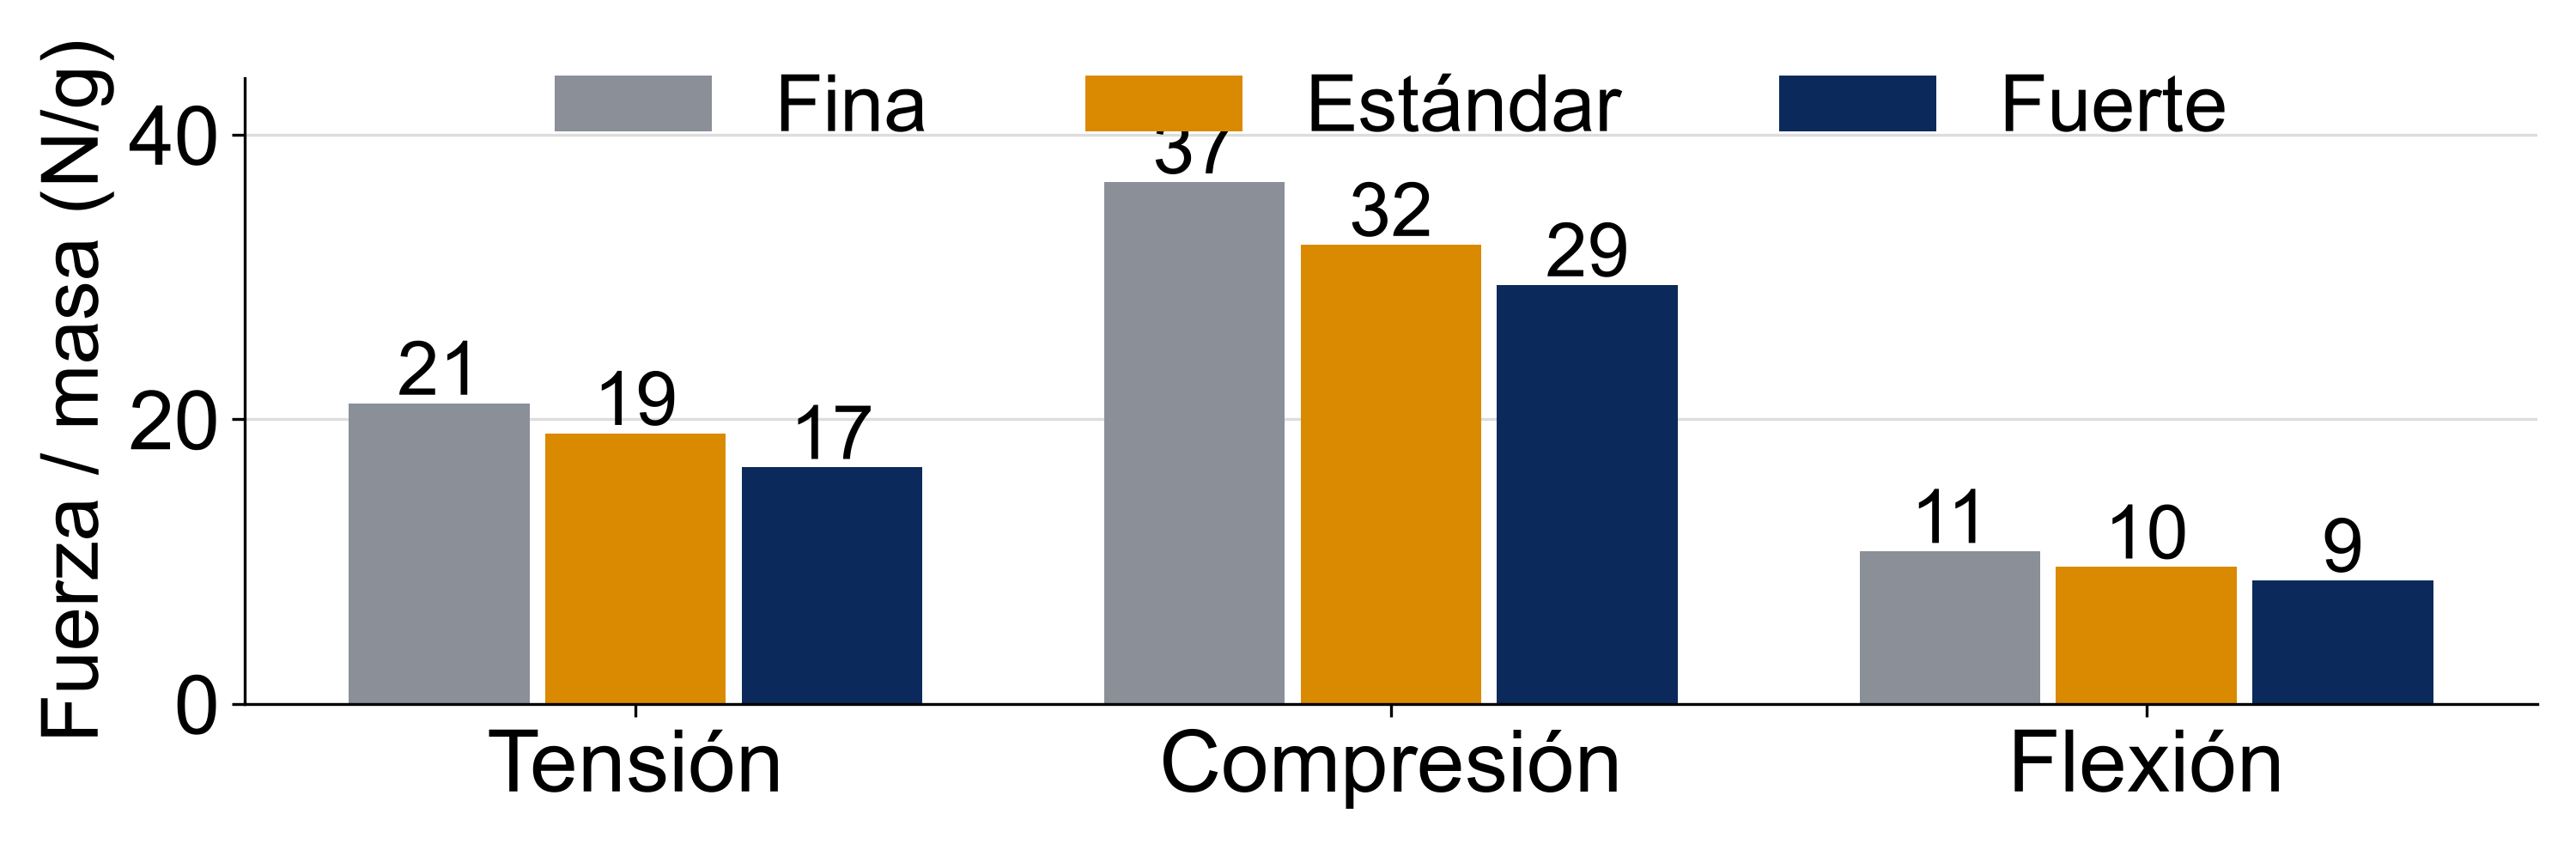
\includegraphics[width=\linewidth]{../figuras/fig4_fuerza_masa.png}\par
{\fontsize{22}{26}\selectfont\textit{Figura 2.} Fuerza máxima por gramo (media de 6 probetas por barra). Fuerte rinde $\approx$20\,\% menos que Fina en este indicador.\par}
\end{minipage}
\end{bloque}
\vspace{3mm}
% ---------------- 5 CONCLUSION ----------------
\enlargethispage{40mm}
\begin{bloque}{5 | Conclusión}
\centering\fontsize{29}{37}\selectfont
\textbf{La orientación horizontal y la configuración Fuerte dieron la mayor carga ({\color{ambar}+64--70\,\%} sobre Fina), pero con 109\,\% más masa y $\approx$20\,\% menos fuerza por gramo: elegir parámetros exige equilibrar carga y material.}
\end{bloque}
\vspace{3mm}
% ---------------- REFERENCIAS ----------------
\begin{bloque}{Referencias clave}
\raggedright\fontsize{20}{23}\selectfont\setlength{\parskip}{4pt}
\begin{minipage}[t]{0.485\linewidth}\vspace{0pt}
Al-Tamimi, A. A., et al. (2023). Investigation and prediction of tensile, flexural, and compressive properties of tough PLA material using definitive screening design. \textit{Polymers, 15}(20), 4169. https://doi.org/10.3390/polym15204169\par
Alafaghani, A., et al. (2017). Experimental optimization of fused deposition modelling processing parameters: A design-for-manufacturing approach. \textit{Procedia Manufacturing, 10}, 791--803. https://doi.org/10.1016/j.promfg.2017.07.079\par
Buss, C., et al. (2026). Experimental investigation into the influence of infill density, print pattern, and built-up direction on the flexural strength of FFF-manufactured PLA components. \textit{Journal of Manufacturing and Materials Processing, 10}(1), 21. https://doi.org/10.3390/jmmp10010021\par
\end{minipage}\hfill
\begin{minipage}[t]{0.485\linewidth}\vspace{0pt}
Chacón, J. M., et al. (2017). Additive manufacturing of PLA structures using fused deposition modelling: Effect of process parameters on mechanical properties and their optimal selection. \textit{Materials \& Design, 124}, 143--157. https://doi.org/10.1016/j.matdes.2017.03.065\par
Ergüder, T. O., \& Bulut, C. (2025). Mechanical characterization of FDM-printed PLA: Role of infill geometry and build direction. \textit{Challenge Journal of Structural Mechanics, 11}(4), 201. https://doi.org/10.20528/cjsmec.2025.04.003\par
\end{minipage}
\end{bloque}
\end{document}
